\section{Исследование и построение решения задачи}
\label{sec:Chapter3} \index{Chapter3}

Согласно главе~\ref{sec:Chapter2}, наилучшие результаты в решении задачи распознавания рукописного текста себя показывают
модели с архитектурой seq2seq и, в частности, трансформеры.
В рамках данной задачи, одним из самых значительных препятствий на пути её решения является недостаток данных,
требуемых для обучения вышеописанных моделей.
В силу трудоёмкости процесса создания большого размеченного набора данных рукописных текстов, применяются техники генерации синтетических данных.
На данный момент предложено несколько подобных техник (см. секцию~\ref{subsubsec:generation}).
Два наиболее известных способа -- это использование рукописных шрифтов и генеративно-состязательных сетей.
Сравнение эффективности использования синтетических данных, сгенерированных различными способами, может позволить понять,
что стоит использовать для получения наилучших результатов.
При этом желательно провести исследование на моделях различных архитектур для того, чтобы избежать
подстраивания экспериментов под особенности конкретной архитектуры.
На текущий момент времени, в существующих научных работах подобного исследования описано не было, насколько это может быть известно.

Если рассматривать задачу распознавания рукописного текста на русском языке,
то здесь сравнение методов расширения наборов данных также является актуальным в силу недостатка научных работ в этой области.
Единственным примером для русского языка служит работа~\cite{shonenkov2021stackmix},
в которой алгоритм генерации полу-синтетических данных Stackmix позволил повысить точность распознавания модели с 71\% до 82\% на наборе HKR.
В дополнение к этому, в научной литературе не упоминается использование самого популярного метода создания синтетических данных
на основе рукописных шрифтов в контексте русского языка.
Реализация подобного метода требует дополнительных исследований.

Таким образом, предлагается рассмотреть некоторые методы генерации синтетических наборов данных и сравнить их в контексте
задачи распознавания рукописного текста на русском языке:
\begin{itemize}
    \item Генерация изображений текста с помощью рукописных шрифтов;
    \item Алгоритм Stackmix для генерации полу-синтетических изображений~\cite{shonenkov2021stackmix};
    \item Генерация изображений рукописного текста при помощи генеративно-состязательных сетей.
\end{itemize}

При этом предлагается рассмотреть две архитектуры нейронных сетей для тестирования методов:
\begin{itemize}
    \item Seq2seq архитектура~\cite{sutskever2014sequence}, состоящая из сверточной и рекуррентных нейронных сетей с механизмом внимания;
    \item Архитектура трансформер~\cite{vaswani2017attention}.
\end{itemize}

Согласно информации из секции~\ref{subsec:datasets}, для русского языка существует два общедоступных эталонных набора данных,
на которых можно проводить исследования.
Они обладают определёнными особенностями и достаточно сильно отличаются друг от друга,
что позволяет более детально проанализировать эффективность методов расширения наборов данных.


\subsection{Генерация изображений текста с помощью рукописных шрифтов}
\label{subsec:synthetic}

Генерация изображений текста с помощью рукописных шрифтов -- наиболее простой способ создания дополнительного обучающего набора данных.
Этот метод не требует обучения дополнительных моделей, не зависит от какого-либо фиксированного набора данных,
прост в реализации и позволяет генерировать данные с большой скоростью.
Несмотря на многочисленные достоинства, генерация текста с помощью шрифтов обладает рядом недостатков.
Типографские шрифты, даже рукописные, не обладают достаточным разнообразием и выглядят искусственно не только для нейронной сети,
но и для человеческого глаза.

Ещё одним существенным недостатком является сложность добавления нового стиля написания, т.е. непосредственно шрифта,
так как, как правило, для этого необходимо большое количество времени и умение работать со специализированным программным обеспечением.
Этот недостаток сильно заметен по отношению к кириллическим шрифтам -- существует не так много открытых рукописных шрифтов, содержащих русские символы.
Поэтому имеет смысл каким-то образом автоматизировать процесс создания нового шрифта.
В этом может помочь приложение \textit{calligraphr}\footnote{\url{https://www.calligraphr.com}},
позволяющее из изображений символов получить шрифт в формате \textit{ttf}.
Изображения рукописных символов можно взять из базы символов, описанной в секции~\ref{subsec:datasets},
в которой для каждого рукописного кириллического символа существует более 1500 вариантов написания.

Приложение \textit{calligraphr} требует заполнения шаблона с заранее выбранным набором символов.
Шаблон представляет собой изображение, содержащее таблицу, в которой в определённых ячейках должны помещаться изображения конкретных символов.
Пример пустого и заполненного шаблона представлен на рисунке~\ref{fig:templates}.

\begin{figure}[h!]
    \centering
    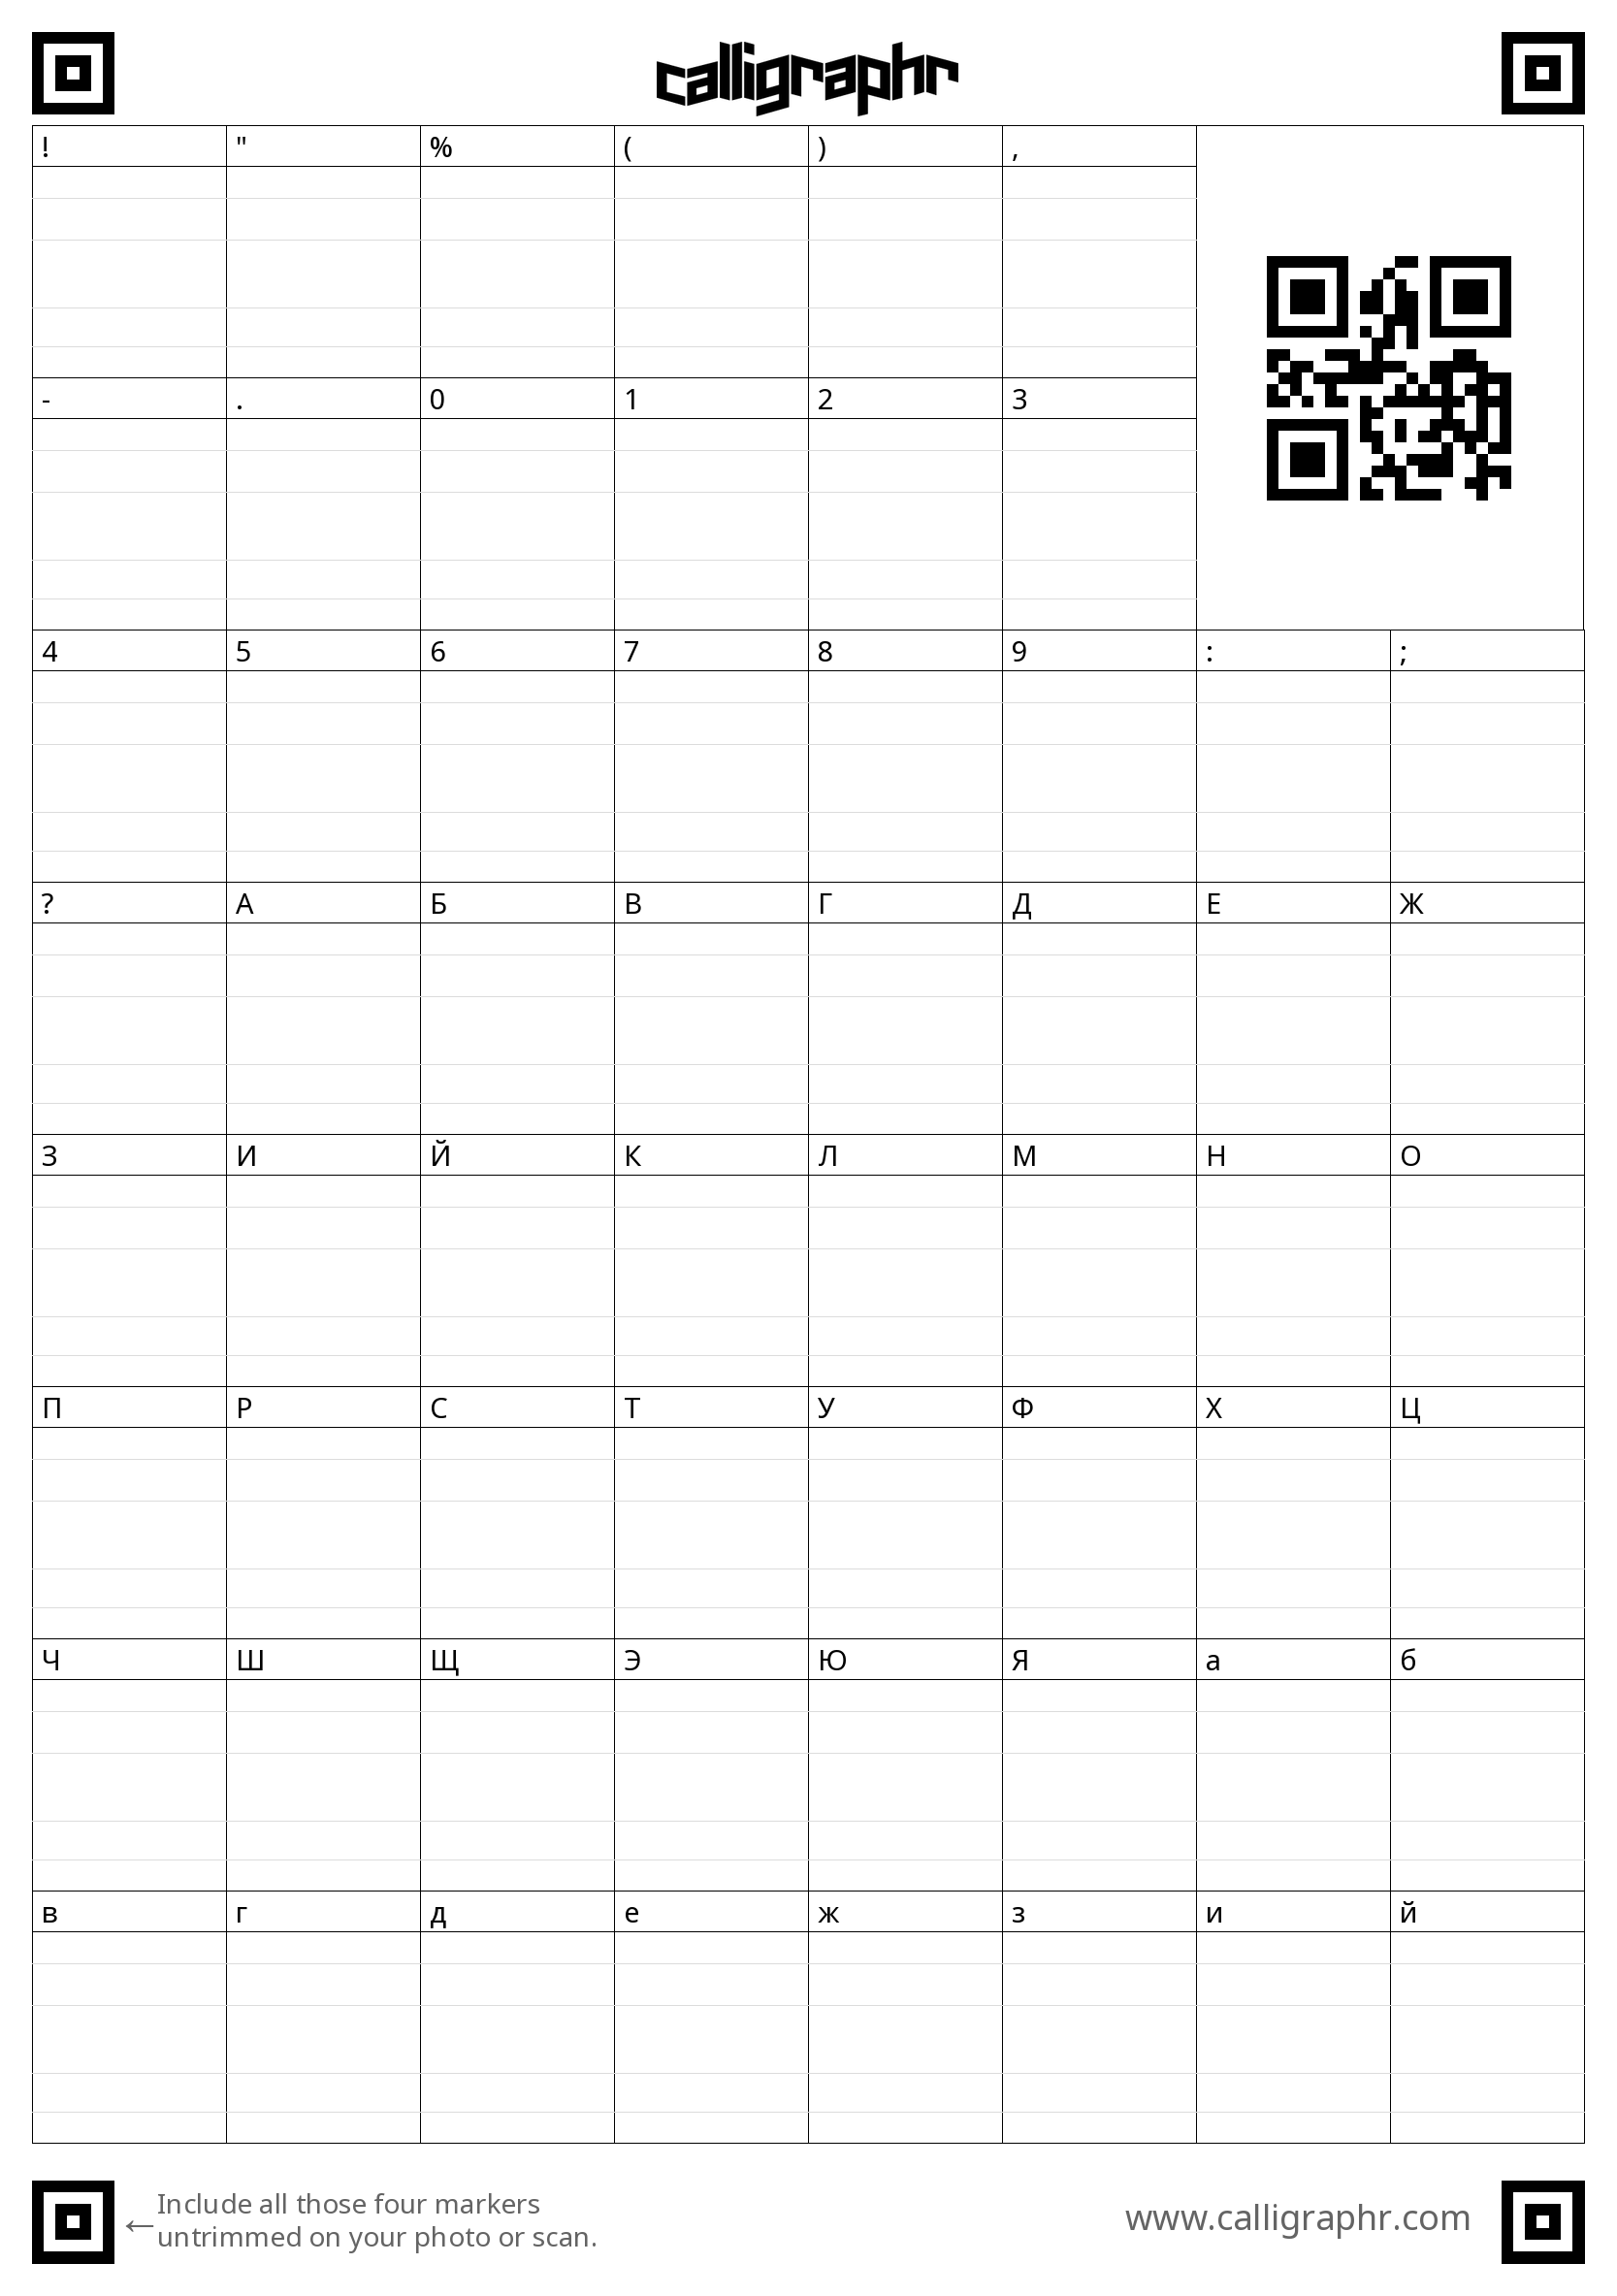
\includegraphics[width=0.45\textwidth]{img/template}
    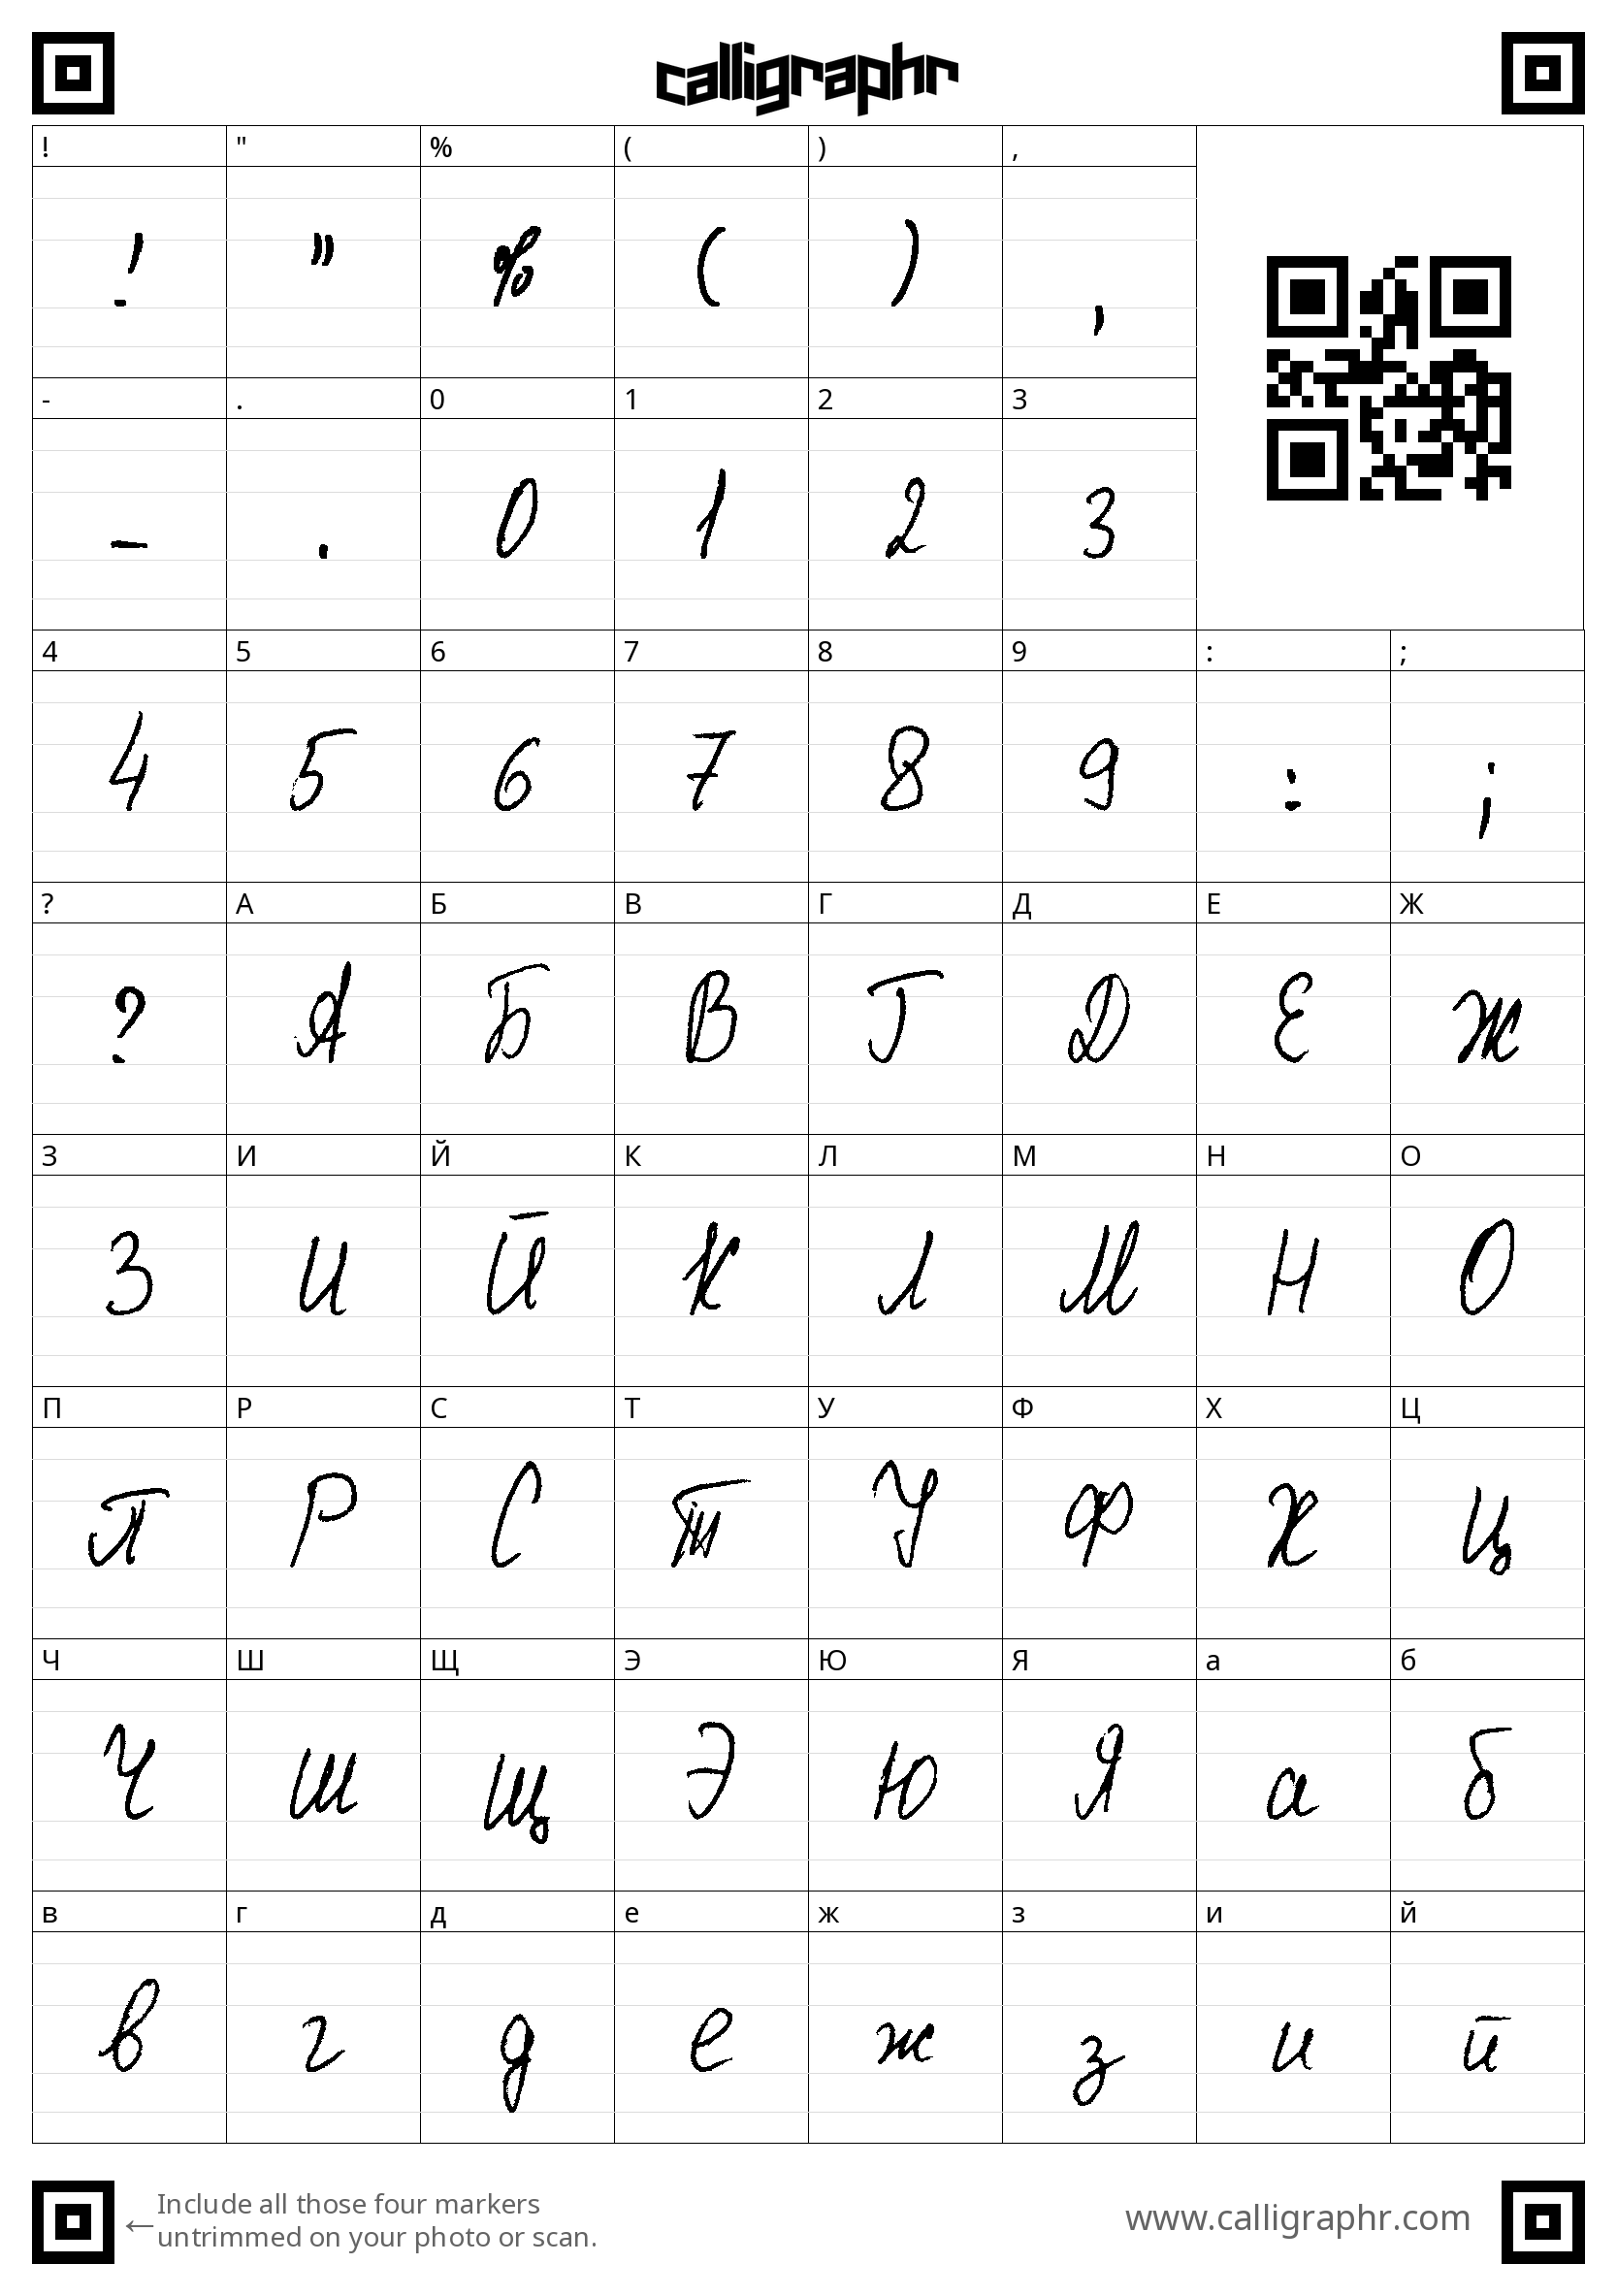
\includegraphics[width=0.45\textwidth]{img/template_filled}
    \caption{Примеры пустого и заполненного шаблонов для приложения \textit{calligraphr}}
    \label{fig:templates}
\end{figure}

Заполненный шаблон далее анализируется приложением, которое извлекает глифы -- векторные изображения символов.
У полученных глифов можно вручную поменять расположение и размер, таким образом прибавив реалистичности к результату.
Затем из глифов формируется шрифт необходимого формата.
Таким образом, создание шрифта можно определенным образом автоматизировать.

Для создания нового кириллического шрифта предлагается следующая последовательность действий:
\begin{enumerate}
    \item Заполнение шаблона для \textit{calligraphr} изображениями кириллических символов;
    \item Ручная коррекция полученных с помощью \textit{calligraphr} глифов при необходимости;
    \item Итоговая сборка шрифта.
\end{enumerate}

Последние два пункта алгоритма выполняются непосредственно с помощью приложения.
Первый пункт требует анализа границ шаблона для поиска координат вставки изображений,
а также нахождения базовой линии символа для того, чтобы вставить его в соответствии с ней.
Границы шаблона можно найти с помощью комбинации морфологических операций \textit{dilate} и \textit{erode},
например, как это сделано для анализа таблиц в библиотеке \textit{dedoc}\footnote{\url{https://github.com/ispras/dedoc}}.
Эти границы можно найти один раз и зафиксировать для конкретного шаблона.
Нахождение базовой линии символа можно с некоторыми оговорками реализовать аналогично нахождению базовой линии слова,
для этого существует метод на основе устойчивой регрессии, описанный в работе~\cite{sueiras2021continuous}.
В силу того, что для символов базовую линию находить сложнее, требуется дополнительная коррекция на втором шаге алгоритма.

Пример одного из шрифтов, полученных с помощью описанного выше алгоритма, представлен на рисунке~\ref{fig:font_example}.

\begin{figure}[h!]
    \centering
    \frame{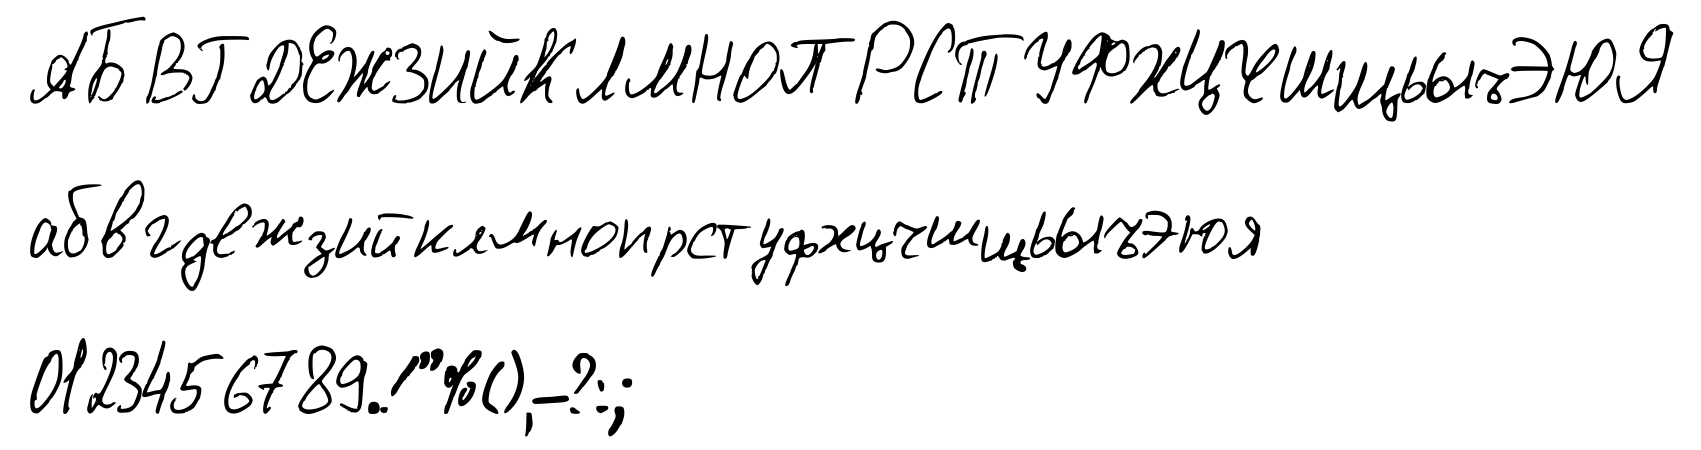
\includegraphics[width=0.8\textwidth]{img/font_example}}
    \caption{Пример шрифта, сгенерированного с помощью приложения \textit{calligraphr} и базы символов}
    \label{fig:font_example}
\end{figure}

Помимо создания новых шрифтов, можно использовать немногочисленные доступные кириллические рукописные шрифты.
При наличии нескольких десятков шрифтов можно реализовать генератор рукописного текста с помощью многочисленных библиотек
отрисовки текста на изображении, и далее создавать достаточно разнообразные синтетические изображения рукописного текста.
Более того, к имеющимся возможностям можно добавить некоторую рандомизацию, напоминающую аугментацию изображений.
При создании изображений можно использовать следующие аугментации:
\begin{itemize}
    \item Изменение размера шрифта, сжатие изображения;
    \item Шумы различных видов (Гауссовский, ISO, мультипликативный);
    \item Размытие различных видов (движения, медианное);
    \item Морфологические операции (эрозия, диляция) для изменения толщины символов;
    \item Изменение наклона шрифта согласно алгоритму из работы~\cite{sueiras2021continuous};
    \item Искажение перспективы изображения;
    \item Небольшие обрезка и повороты изображения;
    \item Имитация рукописных зачеркиваний, описанная в работе~\cite{shonenkov2021stackmix};
    \item Вставка обрезанных символов по краям изображения (имитация соседних строк);
    \item Добавление случайных (светлых, темных) пятен на изображение;
    \item Изменение яркости, контрастности, насыщенности изображения.
\end{itemize}

Таким образом, разработан метод генерации изображений рукописного текста на основе кириллических шрифтов.
Примеры результатов работы генератора рукописного текста представлены на рисунке~\ref{fig:synthetic_example}.

\begin{figure}[h!]
    \centering
    \frame{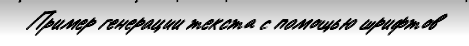
\includegraphics[width=0.9\textwidth]{img/synthetic_cyrillic}}
    \frame{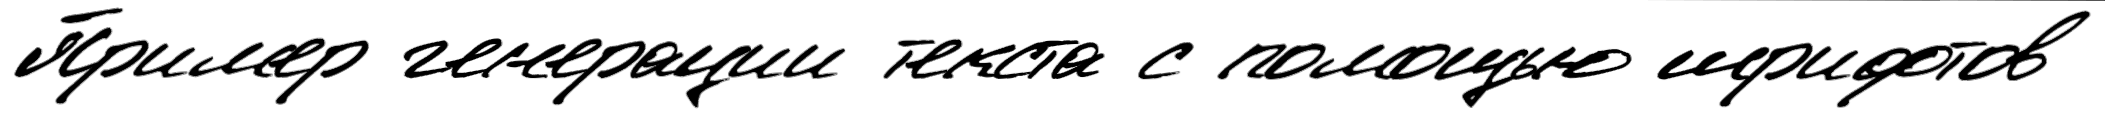
\includegraphics[width=0.9\textwidth]{img/synthetic_hkr}}
    \caption{Примеры результатов работы генератора рукописного текста}
    \label{fig:synthetic_example}
\end{figure}


\subsection{Алгоритм Stackmix для генерации изображений}
\label{subsec:stackmix}

Данный алгоритм генерации синтетических изображений рукописного текста в общих чертах описан в секции~\ref{subsubsec:generation}.
Основной смысл метода заключается в том, что из имеющегося набора данных с фиксированным словарём можно создавать новые слова/предложения
путем нарезки частей имеющих слов и склейки новых слов из этих частей.
Таким образом, метод позволяет модели лучше заточиться под конкретный набор данных, при этом не переобучиваясь на фиксированном наборе слов.
Авторам алгоритма~\cite{shonenkov2021stackmix} удалось существенно поднять качество распознавания предложенной ими модели
на нескольких наборах данных.
Например, благодаря такому расширению наборов, для набора данных HKR точность распознавания увеличилась на 11\%.

Более детально, для того, чтобы использовать метод Stackmix для генерации изображений, нужно выполнить следующую последовательность действий:
\begin{enumerate}
    \item Обучить модель распознавания рукописного текста, предложенную авторами, на обучающем наборе, который планируется расширять;
    \item С помощью обученной на предыдущем шаге модели сгенерировать так называемые символьные маски -- информацию о координатах границ символов в каждом изображении слова из набора данных.
    Эту информацию предоставляет декодер CTC~\cite{graves2008novel}, который является частью предложенной модели.
    \item Сформировать упорядоченный набор обрезанных изображений символов и подслов с настраиваемой максимальной длиной.
    Этот набор будет использоваться для сборки новых слов/предложений из имеющихся нарезок.
    \item Непосредственно запустить алгоритм синтезирования новых слов на основе набора обрезанных изображений символов/подслов.
    Он может быть запущен предварительно на фиксированном корпусе слов, либо использоваться для генерации обучающих примеров во время обучения сети.
\end{enumerate}

Как видно из описания метода, у него есть существенный недостаток -- необходимость в обучении дополнительной модели для получения координат границ символов.
Слово нарезается на символы вертикально -- это означает, что для почерков с наклоном части символов будут обрезаны.
При этом сама модель дает предсказания не со 100\%-ной точностью, что также влияет на качество разделения слов на символы.
И, в дополнение к вышеперечисленному, при склейке нет анализа того, на какой высоте находится очередной символ, поэтому соединения
могут получаться слишком неестественными, а слова -- нечитаемыми.

Несмотря на явные минусы, этот метод всё-таки выполняет свою основную функцию -- набор данных увеличивается довольно
нестандартным способом, который может предотвратить переобучение модели.
При этом, большим плюсом является то, что исходный код метода выложен в открытый доступ\footnote{\url{https://github.com/ai-forever/StackMix-OCR}},
что предоставляет возможность провести эксперименты для проверки эффективности метода.

Примеры результатов работы алгоритма Stackmix на наборах данных HKR и Cyrillic Handwriting Dataset представлены на рисунке~\ref{fig:stackmix_example}.
По примерам, представленным на рисунке, можно сделать вывод, что метод в большей степени подходит для наборов изображений с однородным фоном и
относительно одинаковыми условиями написания текста, что характерно для набора HKR и совершенно несвойственно набору Cyrillic Handwriting Dataset.
Тем не менее, можно попытаться сгладить эффект неоднородности путем предобработки изображений, например, с помощью алгоритмов бинаризации (см. секцию~\ref{subsec:preprocessing}).

\begin{figure}[h!]
    \centering
    \frame{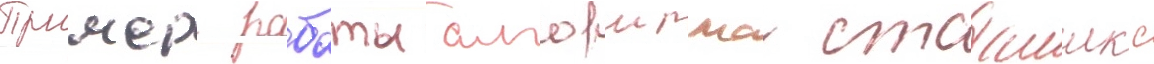
\includegraphics[width=0.9\textwidth]{img/stackmix_hkr}}
    \frame{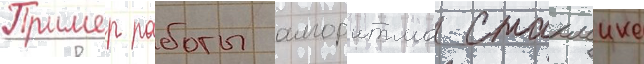
\includegraphics[width=0.9\textwidth]{img/stackmix_cyrillic}}
    \caption{Примеры результатов работы алгоритма Stackmix (сверху для набора HKR, снизу для набора Cyrillic Handwriting Dataset)}
    \label{fig:stackmix_example}
\end{figure}


\subsection{Генерация изображений рукописного текста при помощи\\генеративно-состязательных сетей}
\label{subsec:gan}

Ещё одной популярной областью для исследований в области генерации изображений рукописного текста является применение генеративно-состязательных сетей (GAN).
Согласно описанию секции~\ref{subsubsec:generation}, такие сети в состоят из генеративной модели, создающей примеры,
и дискриминативной модели, отличающей сгенерированные примеры от настоящих.
Здесь, как и в предыдущем описанном методе Stackmix, также есть недостаток оттого, что нужно обучать еще одну модель.
Более того, генеративно-состязательные сети имеют существенно более сложную архитектуру,
вследствие чего требуются значительные ресурсы для их обучения, которые есть далеко не у всех.

Одной из наиболее современных предложенных сетей, генерирующих изображения текста, является ScrabbleGAN~\cite{fogel2020scrabblegan}.
В отличие от остальных известных новейших моделей, ScrabbleGAN имеет относительно несложную структуру и позволяет получать
изображения различных случайных стилей с помощью встроенного вектора шума.
Еще одним существенным достоинством является то, что код модели доступен, причем в разных вариациях,
которые направлены на исправление ошибок и улучшение качества кода.
Следовательно, при наличии достаточных ресурсов для обучения сети, этот метод также воспроизводим.

На рисунке~\ref{fig:gan_example} представлены примеры обученной генеративно-состязательной сети ScrabbleGAN на
наборах данных HKR и Cyrillic Handwriting Dataset.
Как видно из рисунка, изображения получаются достаточно реалистичными, однако некоторые детали соединения символов и фона
дают понять наблюдателю, что данные синтетические.
Аналогично результатам генерации методом Stackmix, изображения для набора данных HKR получаются более удачными по сравнению с
более сложными и вариативными изображениями для Cyrillic Handwriting Dataset.
Стоит также отметить, что в отличие от двух предыдущих описанных методов, генеративно-состязательные сети позволяют
корректно обработать варьирующиеся соединения символов друг с другом.

\begin{figure}[h!]
    \centering
    \frame{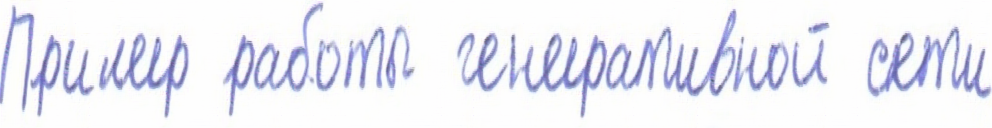
\includegraphics[width=0.9\textwidth]{img/gan_hkr}}
    \frame{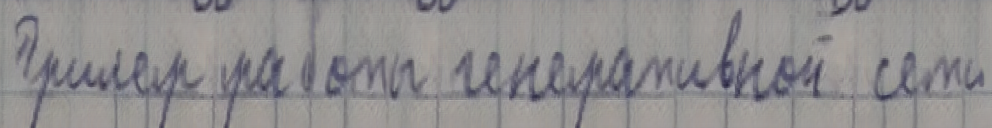
\includegraphics[width=0.9\textwidth]{img/gan_cyrillic}}
    \caption{Примеры результатов работы генеративно-состязательной сети ScrabbleGAN (сверху для набора HKR, снизу для набора Cyrillic Handwriting Dataset)}
    \label{fig:gan_example}
\end{figure}


\subsection{Результаты проведения экспериментов}
\label{subsec:experiments}


